\documentclass{beamer}

\usepackage{graphicx}
\usetheme{Madrid}

\newcommand{\solutionName}{NutrientNexus}

\newif\iflowcort
\lowcorttrue

\title{\solutionName}
\author{Team 38: shakespeareTorta}
\date{\today}
\setbeamertemplate{navigation symbols}{}

\AtBeginSection[]{
    \begin{frame}
        \centering
        \Large \insertsection
    \end{frame}
}


\begin{document}

%---------------------------
% TITLE SLIDE
%---------------------------
\frame{\titlepage}

%---------------------------
% 1. INTRODUCTION (1 slide)
%---------------------------
\begin{frame}{Introduction}
\centering
\textbf{\Huge \solutionName} \\
\vspace{1cm}
\textit{A Digital Twin Autonomous System for Agricultural and Coastal Field
Monitoring and Decision Making}
\end{frame}

\iflowcort
\begin{frame}{Nature of the presentation}
\pause
\centering
\includegraphics[width=\linewidth]{lowcort.png}
\end{frame}
\fi

%---------------------------
% 2. THE PITCH (3 slides)
%---------------------------

\begin{frame}{The Pitch: Aim}
    Autonomous field monitoring and decision-support system. \\
    \pause
    Why?
    \vfill
    \pause

    \textbf{Kill two birds with one stone} \\
    \begin{itemize}
        \item<3-> Holistic, feedback- and context-driven, adaptive crop management system.
        \item<3-> Environment impact baked into the system.
    \end{itemize}
    
    \note{Decision support is the key. We integrate multitude data to propose or
    to enact context aware, minimum-risk decisions.}
\end{frame}

\begin{frame}{The Pitch: Unique Selling Point}
    \textbf{Integrated Digital Twin System} linking farm and coastal
    environments.
    \pause

    \vfill
    Continuous feedback loop
    \begin{itemize}
        \item Real-time weather data
        \item Crop and soil data
        \item Crop growth history
        \item Environment contamination thresholds
        \item Profit margins?
    \end{itemize}
    \pause
    \vfill

    \alert{Bridges gap between agriculture and marine protection.}

    \note{Mention literature pinpointing the importance of decision-oriented
    solutions and disconnected stakeholders. Give an example on how a farmer
    does not know how their fertilisers will affect water basins kilometres
    away.}
\end{frame}

\begin{frame}{The Pitch: SDG Impact}
    Precision in application leads to food safety and lower eutrophication.
    \vfill
    
    \textbf{Feedback driven.}

    \pause
    \vfill
    Who benefits?
    \begin{itemize}
        \item Farmers
        \item Natural habitats
        \item Water ecosystems
    \end{itemize}

    \note{Precision is double-edged sword. With the gathered data, we apply more
    irrigation/fertilisation where it is insufficient -> higher yield, and also
    do not apply when enough. We feed plant growth data into the system so we
    optimise decision-making even further. No need to expland land -> natural
    habitats}
\end{frame}

%---------------------------
% 3. TECHNICAL INSIGHT (2 slides)
%---------------------------

\begin{frame}{Technical Insight: Level 0 Diagram}
\centering
\hspace*{-0.5cm}\includegraphics[width=1.1\textwidth]{level0.png}
\end{frame}

\begin{frame}{Technical Insight: Level 1 Diagram}
\centering
\hspace*{-0.5cm}\includegraphics[width=1.05\textwidth]{newLevel1.png}
\end{frame}

%---------------------------
% 4. CONCEPT MAP (1 slide)
%---------------------------
\iflowcort
\begin{frame}{Concept Map}
\centering
\vspace*{-1cm}\hspace*{-0.3cm}\includegraphics[width=1.05\textwidth]{cmap_old.pdf}
\end{frame}

\begin{frame}{cmap Question}
    Wait, but nothing has changed?
    \pause

    \centering \includegraphics[width=0.7\linewidth]{lowcort_cmap.pdf}
\end{frame}

\fi

\begin{frame}{Concept Map}
\centering
\vspace*{-1cm}\hspace*{-0.3cm}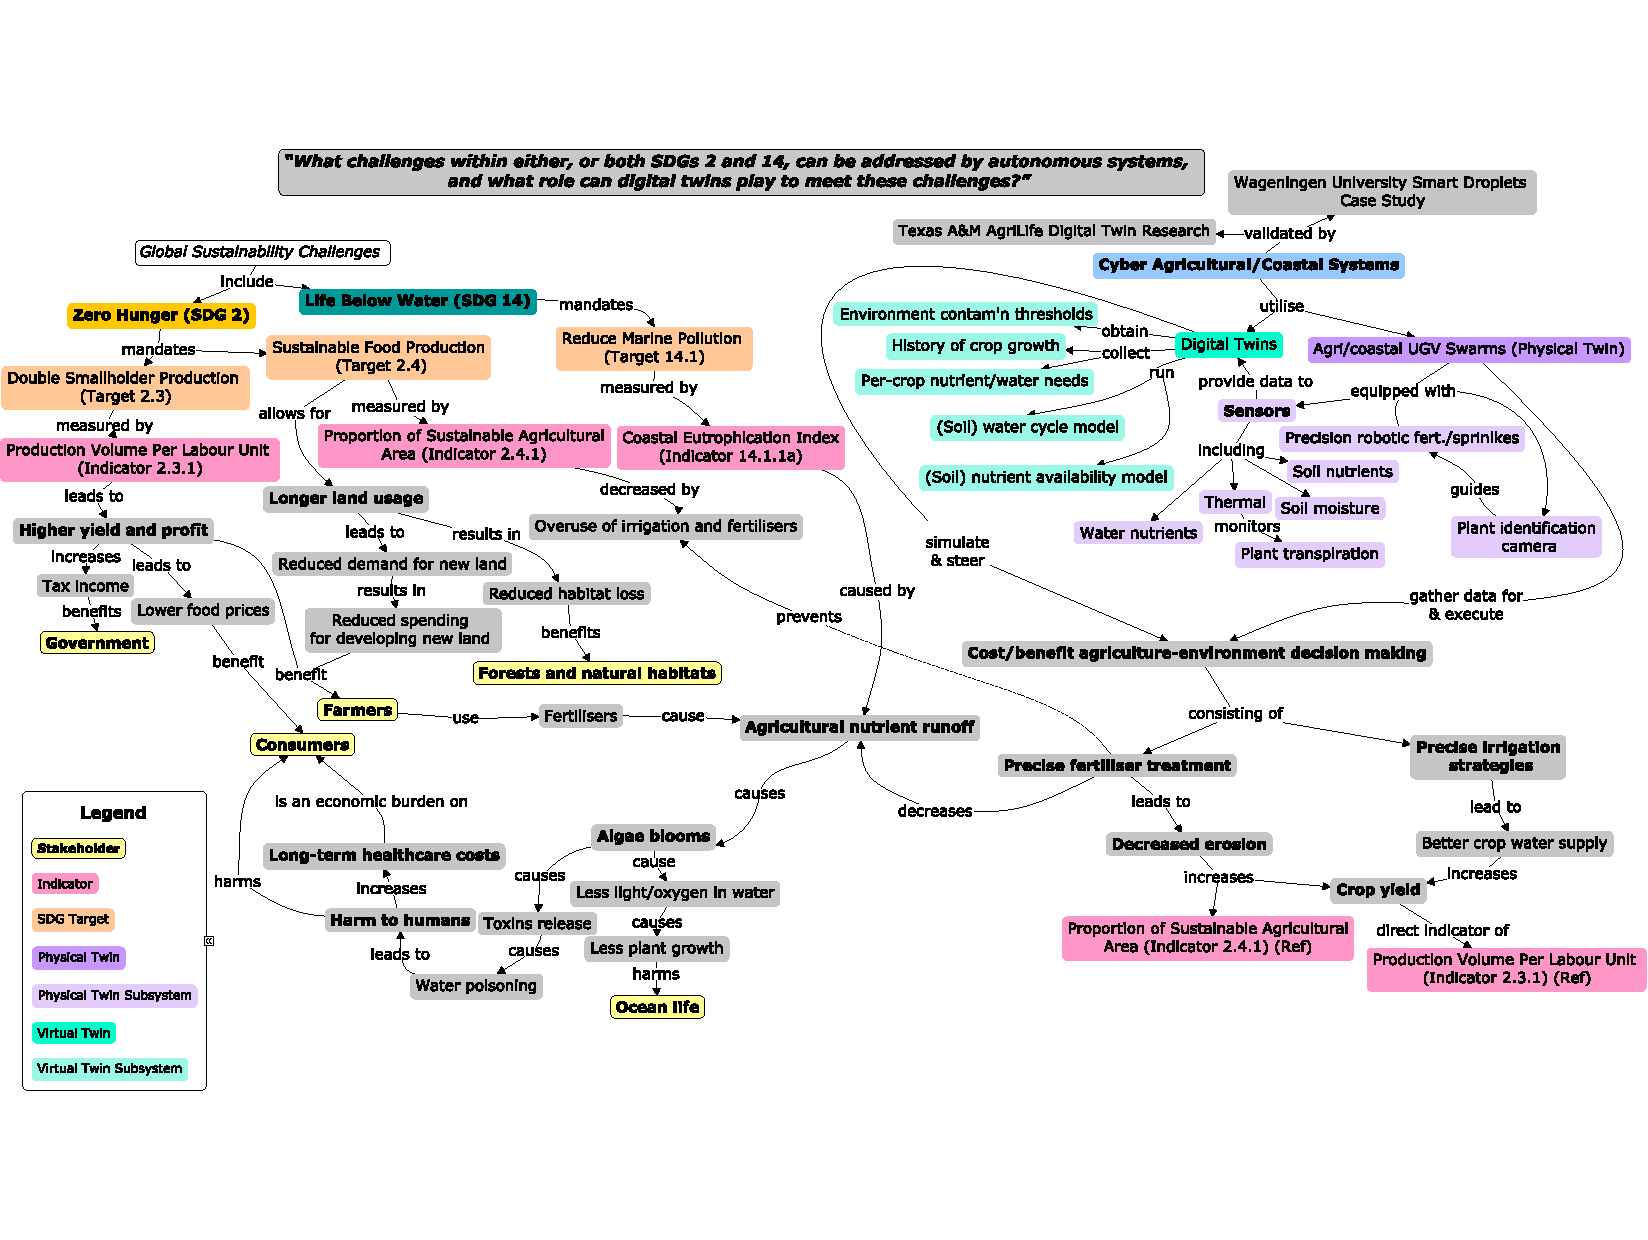
\includegraphics[width=1.05\textwidth]{cmap.pdf}
\end{frame}

\section{Proof of Concept}

\begin{frame}{Overview of the proof of concept}
    \underline{Crop robots only.}
    \pause
    \vfill
    
    Physical twin collects
    \begin{itemize}
        \item Soil water/nutrient level
        \item Past crop growth history
    \end{itemize}
    \vfill

    Digital twin integrates
    \begin{itemize}
        \item Weather + water cycle
        \item Discharge thresholds
        \item Per-crop nutrient/irrigation needs
    \end{itemize}
    \pause
    \vfill

    DT computes optimal fertiliser and irrigation amounts. \\
    Balance between
    \begin{enumerate}
        \item High growth rate
        \item Environment impact
    \end{enumerate}
\end{frame}

\begin{frame}{POC: Implementation detail}
    \textbf{Problem} \\
    Cannot add sensors to Turtlebot.
    \pause
    \vspace{1cm}

    \textbf{Solution} \\
    \emph{Stub out} the sensor getter functions.
\end{frame}

\begin{frame}{PoC: requirements}
    \textbf{Functional}
    \begin{itemize}
        \item Map + navigate crop zones
        \item Digital twin integrate with external data
        \item Optimisation logic balances out yield and environment
    \end{itemize}
    \pause
    \vfill

    \textbf{Non-functional}
    \begin{itemize}
        \item Sycnhronisation between physical and digital twins
        \item Avoid danger zones
        \item Generate concrete recommendations/decisions
    \end{itemize}
\end{frame}

\begin{frame}{PoC: demonstration}
    \begin{itemize}
        \item Field map w/ crop zones
        \item Report (simulated) moisture/nutrient/growth levels
        \item Show one zone with fertiliser advice, another with irrigation
            advice
        \item High-runoff-risk situation where fertiliser is reduced/postponed
        \item Live updates on digital twin during scanning
    \end{itemize}
\end{frame}

\begin{frame}{PoC: resources}
    \begin{itemize}
        \item Turtlebot itself
        \item Software: ROS2, Gazebo, etc.
        \item External data
        \item Domain knowledge
    \end{itemize}
\end{frame}

\begin{frame}{PoC: viability}
    \textbf{Movement} \\
    Can be deployed on the fields, albeit not on harsh terrain.
    \pause
    \vfill

    \textbf{Environment scanning} \\ 
    Essential for decision making. Can be fully emulated/stubbed out.
    \pause
    \vfill

    \textbf{Synchronisation} \\
    Synchronisation possible. Not tested at the planned scale.
\end{frame}

\begin{frame}{PoC: viability}
\centering
\includegraphics[width=\textwidth]{timeline.pdf}
\end{frame}

\end{document}
